% Fig. 1 (system overview), compiled on its own so that the PDF and the Word copy use the same drawing:
% draft/build.sh builds figs/arch.pdf (for LaTeX) and figs/arch.png (for Word) from this file.
\documentclass[border=2pt]{standalone}
\usepackage[T1]{fontenc}
\usepackage{mathptmx}
\usepackage{tikz}
\usetikzlibrary{positioning,arrows.meta,fit}
\begin{document}
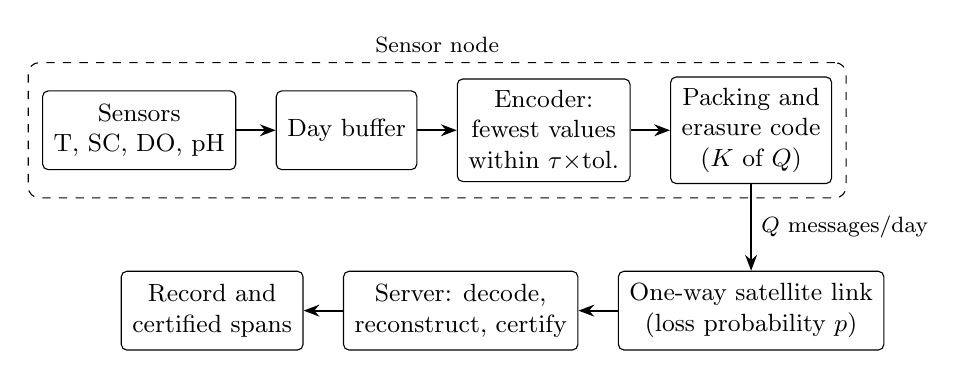
\begin{tikzpicture}[
  box/.style={draw, rounded corners=2pt, align=center, font=\small, minimum height=1.0cm, inner sep=4pt},
  arr/.style={-{Stealth[length=2mm]}, thick}]
\node[box] (s) {Sensors\\T, SC, DO, pH};
\node[box, right=0.5cm of s] (b) {Day buffer};
\node[box, right=0.5cm of b] (e) {Encoder:\\fewest values\\within $\tau\times$tol.};
\node[box, right=0.5cm of e] (c) {Packing and\\erasure code\\($K$ of $Q$)};
\node[box, below=1.1cm of c] (l) {One-way satellite link\\(loss probability $p$)};
\node[box, left=0.5cm of l] (d) {Server: decode,\\reconstruct, certify};
\node[box, left=0.5cm of d] (r) {Record and\\certified spans};
\draw[arr] (s) -- (b);
\draw[arr] (b) -- (e);
\draw[arr] (e) -- (c);
\draw[arr] (c) -- node[right, font=\footnotesize]{$Q$ messages/day} (l);
\draw[arr] (l) -- (d);
\draw[arr] (d) -- (r);
\node[draw, dashed, rounded corners, inner sep=5pt, fit=(s)(b)(e)(c), label={[font=\footnotesize]above:Sensor node}] {};
\end{tikzpicture}
\end{document}
